\documentclass[main]{subfiles}

\begin{document}
    
    \noindent{\Huge SIMULATION}\\
    {\large Algorithm In Action}\\
%----------------------------------------------------------------------------------
    \vspace{15mm}

    \noindent Let's begin with a set of values that we can use for an easy analytical analysis!
        We begin by taking a \textit{diagonally dominant} square matrix $A$ and a known set of values for 
        $\textbf{x}$, which will be the solution of our system $A\textbf{x} = \textbf{b}$ and compute
        $\textbf{b}$ as the matrix product of $A$ and $\textbf{x}$ as $\textbf{b} = A\textbf{x}$:

        \begin{equation}   
            \textit{taking, } \hspace{10mm} A = \begin{bmatrix}
                10 & 2 & 4 & -1 \\
                3 & 11 & 5 & 3 \\
                1 & -2 & -15 &-4 \\
                2 & -2 & 4 & 12 
            \end{bmatrix},\hspace{2mm}
            \textbf{x} = \begin{bmatrix}
                1 \\
                2 \\
                3 \\
                4 \\
            \end{bmatrix}
            \hspace{2mm}
        \implies \textbf{b} = \begin{bmatrix}
                22 \\
                52 \\
                -64\\
                58 \\
            \end{bmatrix}
        \end{equation}
%----------------------------------------------------------------------------------
\vspace{10mm}
\\
The above $A$ and $\textbf{b}$ represent the following system of equations in $\textbf{x} = (x_1, x_2, x_3, x_4)$  

\begin{align}
    10 x_1 + 2 x_2 + 4 x_3     -  x_4  &= 22        \\
    3  x_1 + 11 x_2  + 5  x_3  + 3  x_4 &= 52   \\
      x_1 - 2 x_2   - 15 x_3  - 4  x_4 &= -64   \\
    2  x_1 - 2 x_2   + 4  x_3  + 12 x_4 &= 58
\end{align}
\\
whose exact or true solution is:

\[
    \textbf{x}_t = \begin{bmatrix}
        1 \\
        2 \\
        3 \\
        4 \\
    \end{bmatrix}
\]

\clearpage

%----------------------------------------------------------------------------------


    \subfile{code} 


%----------------------------------------------------------------------------------
    \begin{figure}[t!]
    We now pass $A$ and $\textbf{b}$ to our program \textit{Solve\_Lin\_Alg\_Jacobi\_method.m}
    and solve for $\textbf{x}$ with various tolerances:
    \vspace{2mm}
    \end{figure}


    Figure 1 shows a screenshot of the program run with tolerance set to $0.1$. 
    The output is our solution $\textbf{x}$, $\textbf{x}_t$ is the true solution 
    and $\epsilon_0$ accounts for the error in caclulation:
    
    \begin{figure}
        \makebox[\textwidth][c]{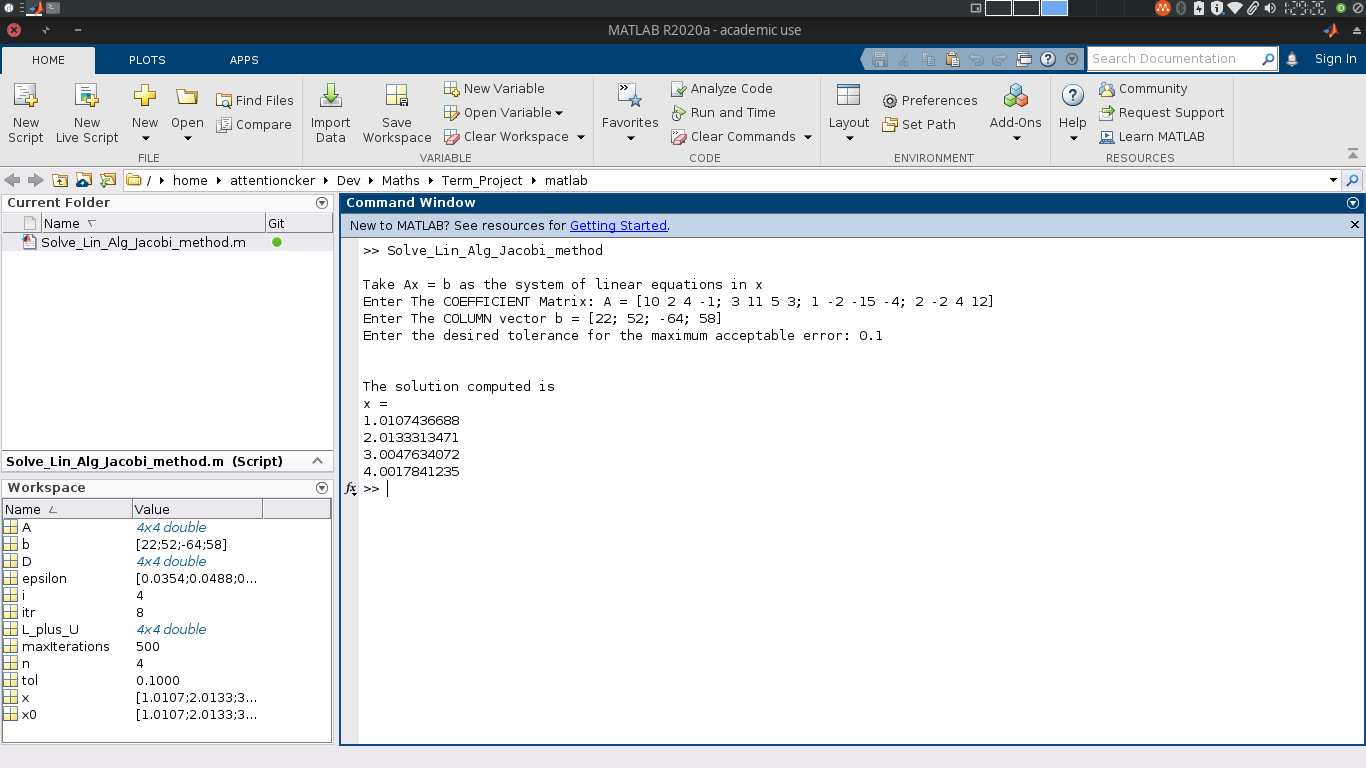
\includegraphics[width=1.4\textwidth]{tol1}}%
        \caption{Tolerance set to 0.1}\label{fig:key}
    \end{figure}
    
    \begin{equation*}
        \textbf{x} = \begin{bmatrix}
            1.0107436688\\
            2.0133313471\\
            3.0047634072\\
            4.0017841235\\
        \end{bmatrix},
        \hspace{3mm}\textit{true solution }\textbf{x}_t = \begin{bmatrix}
            1\\
            2\\
            3\\
            4
        \end{bmatrix}
        \implies max\:error, \epsilon_0 = 0.0133313471
    \end{equation*}
    
\clearpage
%----------------------------------------------------------------------------------

    \begin{figure}[t!]
        \makebox[\textwidth][c]{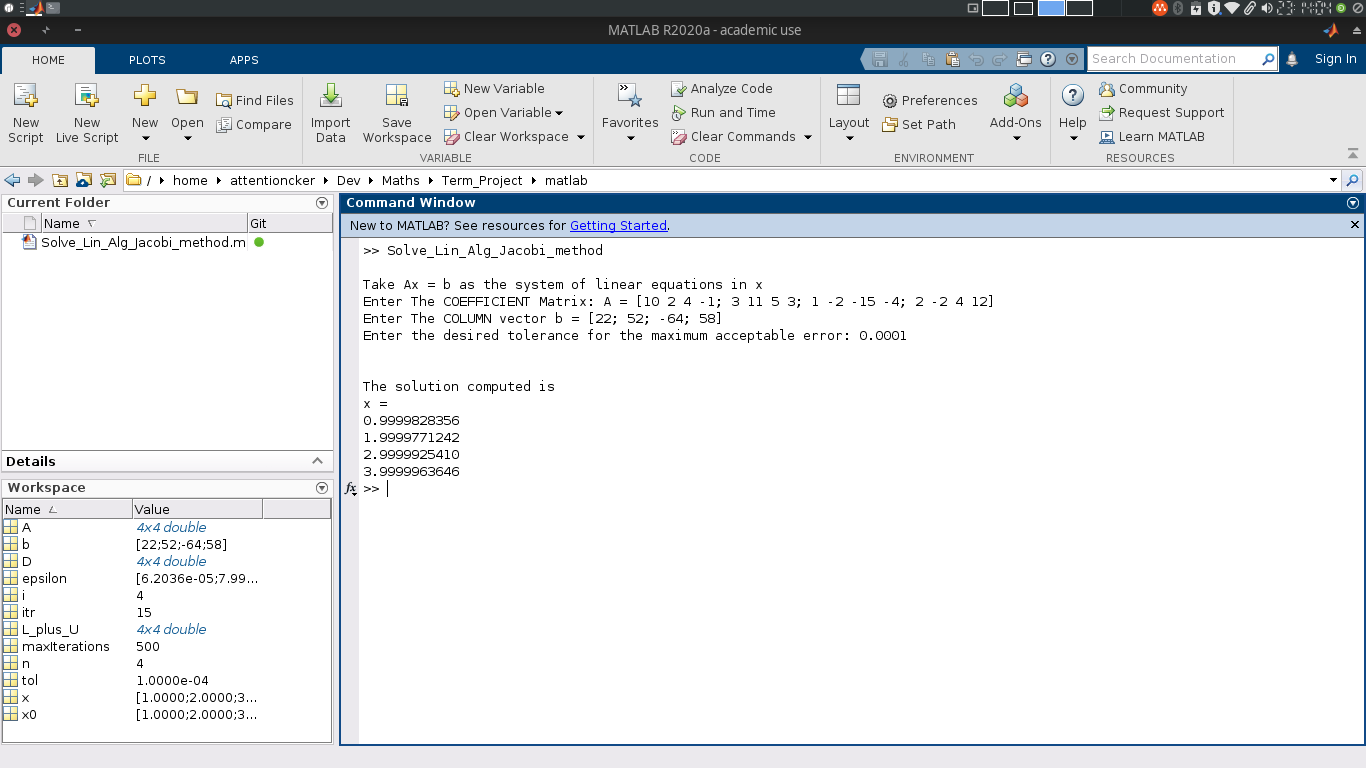
\includegraphics[width=1.4\textwidth]{tol4}}%
        \caption{Tolerance set to 0.0001}\label{fig:key}
    \end{figure}

    Figure 2 shows a screenshot of the program run with tolerance set to $0.1$. 
    The output is our solution $\textbf{x}$, $\textbf{x}_t$ is the true solution 
    and $\epsilon_0$ accounts for the error in caclulation:
    
    \begin{equation*}
        \textbf{x} = \begin{bmatrix}
            0.9999828356\\
            1.9999771242\\
            2.9999925410\\
            3.9999963646\\
        \end{bmatrix},
        \hspace{3mm}\textit{true solution }\textbf{x}_t = \begin{bmatrix}
            1\\
            2\\
            3\\
            4
        \end{bmatrix}
        \implies max error, \epsilon_0 = 0.0000228758
    \end{equation*}
    \clearpage
%----------------------------------------------------------------------------------

    \begin{figure}[t!]
        \makebox[\textwidth][c]{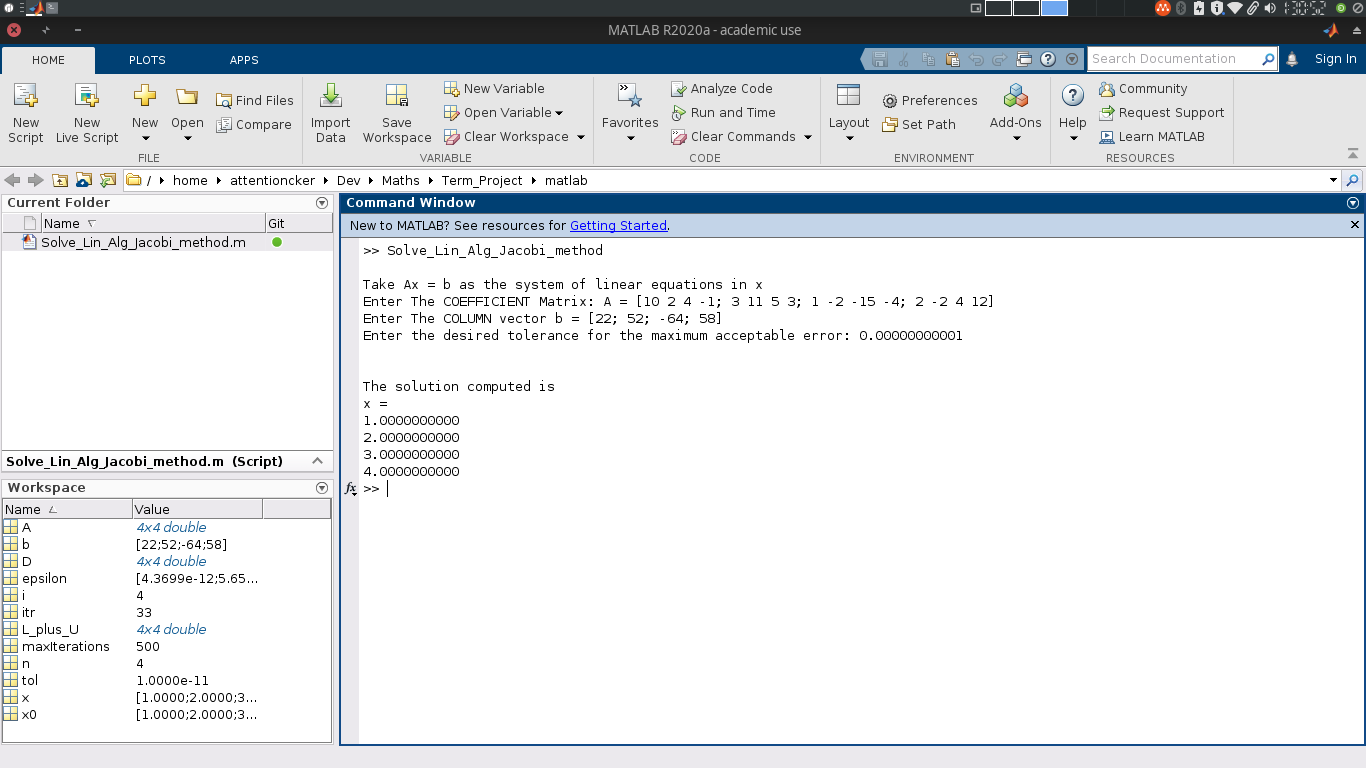
\includegraphics[width=1.4\textwidth]{tol10}}%
        \caption{Tolerance set to 0.00000000001}\label{fig:key}
    \end{figure}

    Figure 3 shows a screenshot of the program run with tolerance set to $0.00000000001$. 
    The output is our solution $\textbf{x}$, $\textbf{x}_t$ is the true solution 
    and $\epsilon_0$ accounts for the error in caclulation:
    
    \begin{equation*}
        \textbf{x} = \begin{bmatrix}
            1.0000000000\\
            2.0000000000\\
            3.0000000000\\
            4.0000000000\\
        \end{bmatrix},
        \hspace{3mm}\textit{true solution }\textbf{x}_t = \begin{bmatrix}
            1\\
            2\\
            3\\
            4
        \end{bmatrix}
        \implies max error, \epsilon_0 = 0.0000000000
    \end{equation*}
    \clearpage
%----------------------------------------------------------------------------------

\clearpage

\end{document}
